% Generated by Sphinx.
\def\sphinxdocclass{report}
\documentclass[letterpaper,10pt,english]{sphinxmanual}
\usepackage[utf8]{inputenc}
\DeclareUnicodeCharacter{00A0}{\nobreakspace}
\usepackage[T1]{fontenc}
\usepackage{babel}
\usepackage{times}
\usepackage[Bjarne]{fncychap}
\usepackage{longtable}
\usepackage{sphinx}
\usepackage{multirow}


\title{Pyfrid Documentation}
\date{June 01, 2012}
\release{0.1.1}
\author{Denis Korolkov}
\newcommand{\sphinxlogo}{}
\renewcommand{\releasename}{Release}
\makeindex

\makeatletter
\def\PYG@reset{\let\PYG@it=\relax \let\PYG@bf=\relax%
    \let\PYG@ul=\relax \let\PYG@tc=\relax%
    \let\PYG@bc=\relax \let\PYG@ff=\relax}
\def\PYG@tok#1{\csname PYG@tok@#1\endcsname}
\def\PYG@toks#1+{\ifx\relax#1\empty\else%
    \PYG@tok{#1}\expandafter\PYG@toks\fi}
\def\PYG@do#1{\PYG@bc{\PYG@tc{\PYG@ul{%
    \PYG@it{\PYG@bf{\PYG@ff{#1}}}}}}}
\def\PYG#1#2{\PYG@reset\PYG@toks#1+\relax+\PYG@do{#2}}

\expandafter\def\csname PYG@tok@gd\endcsname{\def\PYG@tc##1{\textcolor[rgb]{0.63,0.00,0.00}{##1}}}
\expandafter\def\csname PYG@tok@gu\endcsname{\let\PYG@bf=\textbf\def\PYG@tc##1{\textcolor[rgb]{0.50,0.00,0.50}{##1}}}
\expandafter\def\csname PYG@tok@gt\endcsname{\def\PYG@tc##1{\textcolor[rgb]{0.00,0.25,0.82}{##1}}}
\expandafter\def\csname PYG@tok@gs\endcsname{\let\PYG@bf=\textbf}
\expandafter\def\csname PYG@tok@gr\endcsname{\def\PYG@tc##1{\textcolor[rgb]{1.00,0.00,0.00}{##1}}}
\expandafter\def\csname PYG@tok@cm\endcsname{\let\PYG@it=\textit\def\PYG@tc##1{\textcolor[rgb]{0.25,0.50,0.56}{##1}}}
\expandafter\def\csname PYG@tok@vg\endcsname{\def\PYG@tc##1{\textcolor[rgb]{0.73,0.38,0.84}{##1}}}
\expandafter\def\csname PYG@tok@m\endcsname{\def\PYG@tc##1{\textcolor[rgb]{0.13,0.50,0.31}{##1}}}
\expandafter\def\csname PYG@tok@mh\endcsname{\def\PYG@tc##1{\textcolor[rgb]{0.13,0.50,0.31}{##1}}}
\expandafter\def\csname PYG@tok@cs\endcsname{\def\PYG@tc##1{\textcolor[rgb]{0.25,0.50,0.56}{##1}}\def\PYG@bc##1{\setlength{\fboxsep}{0pt}\colorbox[rgb]{1.00,0.94,0.94}{\strut ##1}}}
\expandafter\def\csname PYG@tok@ge\endcsname{\let\PYG@it=\textit}
\expandafter\def\csname PYG@tok@vc\endcsname{\def\PYG@tc##1{\textcolor[rgb]{0.73,0.38,0.84}{##1}}}
\expandafter\def\csname PYG@tok@il\endcsname{\def\PYG@tc##1{\textcolor[rgb]{0.13,0.50,0.31}{##1}}}
\expandafter\def\csname PYG@tok@go\endcsname{\def\PYG@tc##1{\textcolor[rgb]{0.19,0.19,0.19}{##1}}}
\expandafter\def\csname PYG@tok@cp\endcsname{\def\PYG@tc##1{\textcolor[rgb]{0.00,0.44,0.13}{##1}}}
\expandafter\def\csname PYG@tok@gi\endcsname{\def\PYG@tc##1{\textcolor[rgb]{0.00,0.63,0.00}{##1}}}
\expandafter\def\csname PYG@tok@gh\endcsname{\let\PYG@bf=\textbf\def\PYG@tc##1{\textcolor[rgb]{0.00,0.00,0.50}{##1}}}
\expandafter\def\csname PYG@tok@ni\endcsname{\let\PYG@bf=\textbf\def\PYG@tc##1{\textcolor[rgb]{0.84,0.33,0.22}{##1}}}
\expandafter\def\csname PYG@tok@nl\endcsname{\let\PYG@bf=\textbf\def\PYG@tc##1{\textcolor[rgb]{0.00,0.13,0.44}{##1}}}
\expandafter\def\csname PYG@tok@nn\endcsname{\let\PYG@bf=\textbf\def\PYG@tc##1{\textcolor[rgb]{0.05,0.52,0.71}{##1}}}
\expandafter\def\csname PYG@tok@no\endcsname{\def\PYG@tc##1{\textcolor[rgb]{0.38,0.68,0.84}{##1}}}
\expandafter\def\csname PYG@tok@na\endcsname{\def\PYG@tc##1{\textcolor[rgb]{0.25,0.44,0.63}{##1}}}
\expandafter\def\csname PYG@tok@nb\endcsname{\def\PYG@tc##1{\textcolor[rgb]{0.00,0.44,0.13}{##1}}}
\expandafter\def\csname PYG@tok@nc\endcsname{\let\PYG@bf=\textbf\def\PYG@tc##1{\textcolor[rgb]{0.05,0.52,0.71}{##1}}}
\expandafter\def\csname PYG@tok@nd\endcsname{\let\PYG@bf=\textbf\def\PYG@tc##1{\textcolor[rgb]{0.33,0.33,0.33}{##1}}}
\expandafter\def\csname PYG@tok@ne\endcsname{\def\PYG@tc##1{\textcolor[rgb]{0.00,0.44,0.13}{##1}}}
\expandafter\def\csname PYG@tok@nf\endcsname{\def\PYG@tc##1{\textcolor[rgb]{0.02,0.16,0.49}{##1}}}
\expandafter\def\csname PYG@tok@si\endcsname{\let\PYG@it=\textit\def\PYG@tc##1{\textcolor[rgb]{0.44,0.63,0.82}{##1}}}
\expandafter\def\csname PYG@tok@s2\endcsname{\def\PYG@tc##1{\textcolor[rgb]{0.25,0.44,0.63}{##1}}}
\expandafter\def\csname PYG@tok@vi\endcsname{\def\PYG@tc##1{\textcolor[rgb]{0.73,0.38,0.84}{##1}}}
\expandafter\def\csname PYG@tok@nt\endcsname{\let\PYG@bf=\textbf\def\PYG@tc##1{\textcolor[rgb]{0.02,0.16,0.45}{##1}}}
\expandafter\def\csname PYG@tok@nv\endcsname{\def\PYG@tc##1{\textcolor[rgb]{0.73,0.38,0.84}{##1}}}
\expandafter\def\csname PYG@tok@s1\endcsname{\def\PYG@tc##1{\textcolor[rgb]{0.25,0.44,0.63}{##1}}}
\expandafter\def\csname PYG@tok@gp\endcsname{\let\PYG@bf=\textbf\def\PYG@tc##1{\textcolor[rgb]{0.78,0.36,0.04}{##1}}}
\expandafter\def\csname PYG@tok@sh\endcsname{\def\PYG@tc##1{\textcolor[rgb]{0.25,0.44,0.63}{##1}}}
\expandafter\def\csname PYG@tok@ow\endcsname{\let\PYG@bf=\textbf\def\PYG@tc##1{\textcolor[rgb]{0.00,0.44,0.13}{##1}}}
\expandafter\def\csname PYG@tok@sx\endcsname{\def\PYG@tc##1{\textcolor[rgb]{0.78,0.36,0.04}{##1}}}
\expandafter\def\csname PYG@tok@bp\endcsname{\def\PYG@tc##1{\textcolor[rgb]{0.00,0.44,0.13}{##1}}}
\expandafter\def\csname PYG@tok@c1\endcsname{\let\PYG@it=\textit\def\PYG@tc##1{\textcolor[rgb]{0.25,0.50,0.56}{##1}}}
\expandafter\def\csname PYG@tok@kc\endcsname{\let\PYG@bf=\textbf\def\PYG@tc##1{\textcolor[rgb]{0.00,0.44,0.13}{##1}}}
\expandafter\def\csname PYG@tok@c\endcsname{\let\PYG@it=\textit\def\PYG@tc##1{\textcolor[rgb]{0.25,0.50,0.56}{##1}}}
\expandafter\def\csname PYG@tok@mf\endcsname{\def\PYG@tc##1{\textcolor[rgb]{0.13,0.50,0.31}{##1}}}
\expandafter\def\csname PYG@tok@err\endcsname{\def\PYG@bc##1{\setlength{\fboxsep}{0pt}\fcolorbox[rgb]{1.00,0.00,0.00}{1,1,1}{\strut ##1}}}
\expandafter\def\csname PYG@tok@kd\endcsname{\let\PYG@bf=\textbf\def\PYG@tc##1{\textcolor[rgb]{0.00,0.44,0.13}{##1}}}
\expandafter\def\csname PYG@tok@ss\endcsname{\def\PYG@tc##1{\textcolor[rgb]{0.32,0.47,0.09}{##1}}}
\expandafter\def\csname PYG@tok@sr\endcsname{\def\PYG@tc##1{\textcolor[rgb]{0.14,0.33,0.53}{##1}}}
\expandafter\def\csname PYG@tok@mo\endcsname{\def\PYG@tc##1{\textcolor[rgb]{0.13,0.50,0.31}{##1}}}
\expandafter\def\csname PYG@tok@mi\endcsname{\def\PYG@tc##1{\textcolor[rgb]{0.13,0.50,0.31}{##1}}}
\expandafter\def\csname PYG@tok@kn\endcsname{\let\PYG@bf=\textbf\def\PYG@tc##1{\textcolor[rgb]{0.00,0.44,0.13}{##1}}}
\expandafter\def\csname PYG@tok@o\endcsname{\def\PYG@tc##1{\textcolor[rgb]{0.40,0.40,0.40}{##1}}}
\expandafter\def\csname PYG@tok@kr\endcsname{\let\PYG@bf=\textbf\def\PYG@tc##1{\textcolor[rgb]{0.00,0.44,0.13}{##1}}}
\expandafter\def\csname PYG@tok@s\endcsname{\def\PYG@tc##1{\textcolor[rgb]{0.25,0.44,0.63}{##1}}}
\expandafter\def\csname PYG@tok@kp\endcsname{\def\PYG@tc##1{\textcolor[rgb]{0.00,0.44,0.13}{##1}}}
\expandafter\def\csname PYG@tok@w\endcsname{\def\PYG@tc##1{\textcolor[rgb]{0.73,0.73,0.73}{##1}}}
\expandafter\def\csname PYG@tok@kt\endcsname{\def\PYG@tc##1{\textcolor[rgb]{0.56,0.13,0.00}{##1}}}
\expandafter\def\csname PYG@tok@sc\endcsname{\def\PYG@tc##1{\textcolor[rgb]{0.25,0.44,0.63}{##1}}}
\expandafter\def\csname PYG@tok@sb\endcsname{\def\PYG@tc##1{\textcolor[rgb]{0.25,0.44,0.63}{##1}}}
\expandafter\def\csname PYG@tok@k\endcsname{\let\PYG@bf=\textbf\def\PYG@tc##1{\textcolor[rgb]{0.00,0.44,0.13}{##1}}}
\expandafter\def\csname PYG@tok@se\endcsname{\let\PYG@bf=\textbf\def\PYG@tc##1{\textcolor[rgb]{0.25,0.44,0.63}{##1}}}
\expandafter\def\csname PYG@tok@sd\endcsname{\let\PYG@it=\textit\def\PYG@tc##1{\textcolor[rgb]{0.25,0.44,0.63}{##1}}}

\def\PYGZbs{\char`\\}
\def\PYGZus{\char`\_}
\def\PYGZob{\char`\{}
\def\PYGZcb{\char`\}}
\def\PYGZca{\char`\^}
\def\PYGZam{\char`\&}
\def\PYGZlt{\char`\<}
\def\PYGZgt{\char`\>}
\def\PYGZsh{\char`\#}
\def\PYGZpc{\char`\%}
\def\PYGZdl{\char`\$}
\def\PYGZti{\char`\~}
% for compatibility with earlier versions
\def\PYGZat{@}
\def\PYGZlb{[}
\def\PYGZrb{]}
\makeatother

\begin{document}

\maketitle
\tableofcontents
\phantomsection\label{index::doc}


Contents:


\chapter{Introduction}
\label{intro:introduction}\label{intro::doc}\label{intro:welcome-to-pyfrid-s-documentation}
This is the documentation for PyFRID, Python Framework for an Instrument Development.
PyFRID is a tool for creating versatile flexible applications for an instrument from simple
laboratory setup, to something more complex like neutron or X-ray diffractometer.
That is, if you have a bunch of motors, sensors, detectors or any other hardware and would like
to manipulate them, to program their behavior, to test them and represent information from them in a convinient way,
PyFRID will give you these capabilities and will organize your hardware under a command line application
or a web-based Graphical User Interface.
\begin{figure}[htbp]\begin{flushright}
\capstart

\scalebox{0.300000}{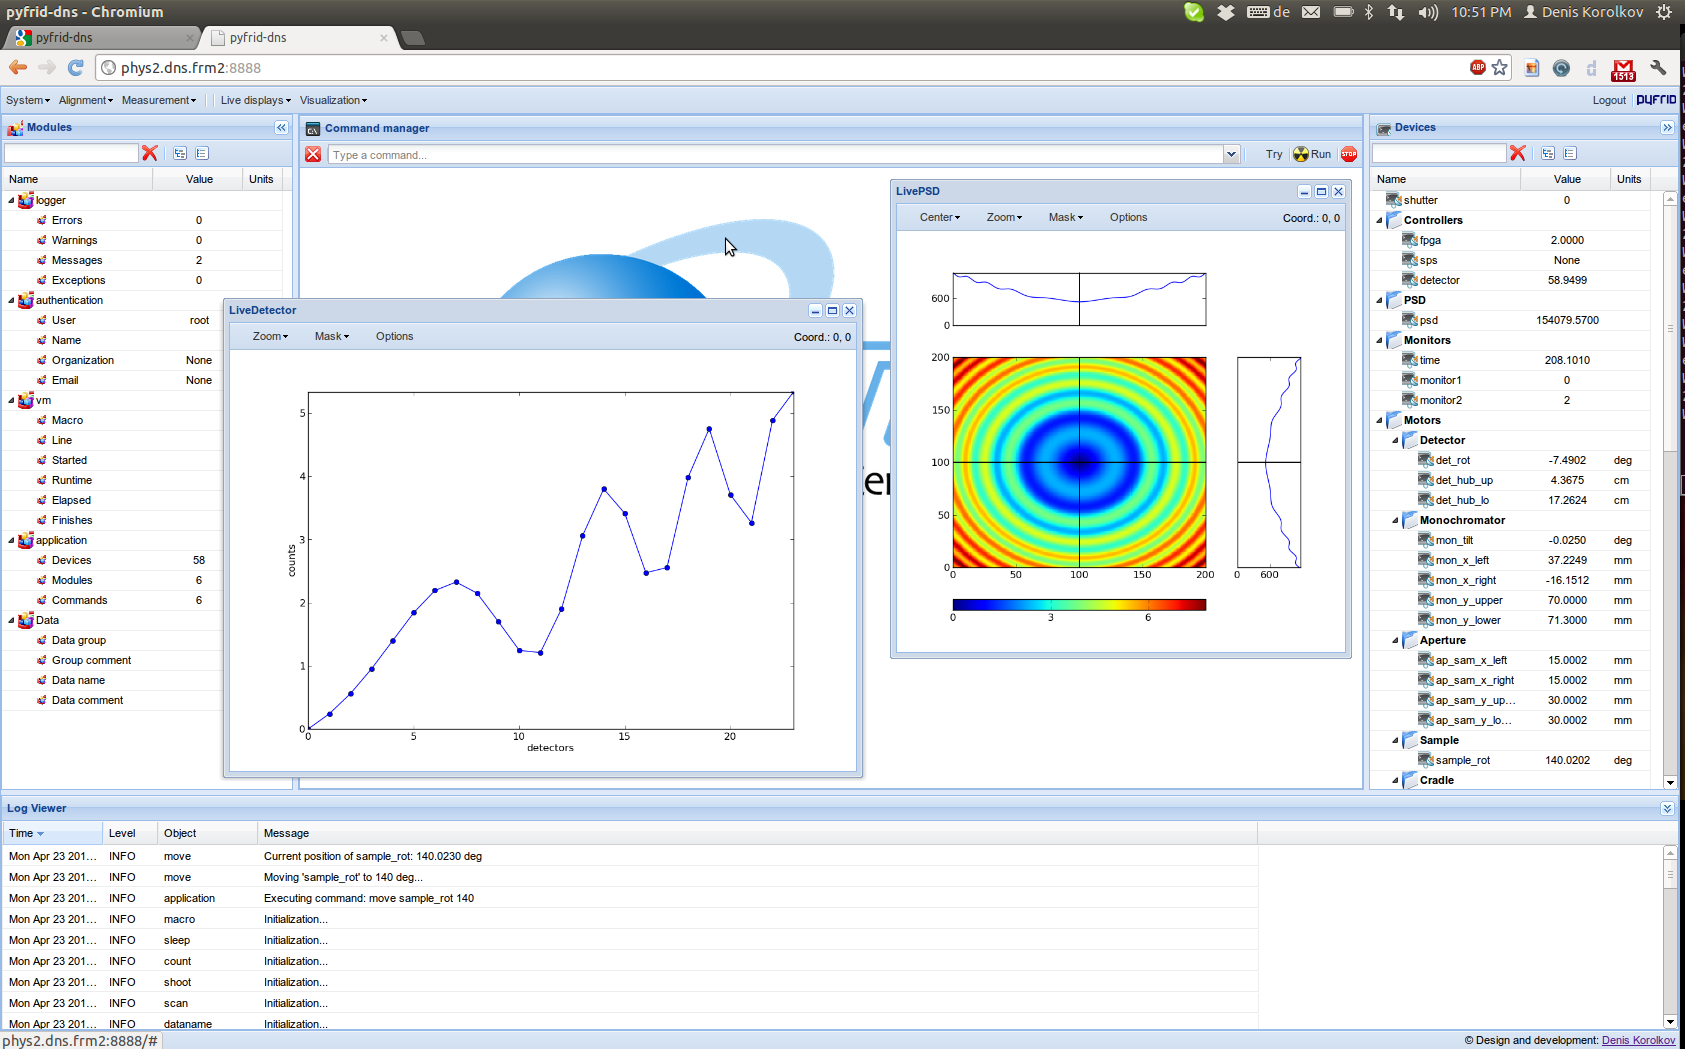
\includegraphics{web.png}}
\caption{Web interface of application created with PyFRID}\end{flushright}\end{figure}

Pyfrid is a modular framework. The building blocks of PyFRID are devices, commands and modules.

The central part of PyFRID is a simple script language. The script language consists of commands,
which give control over the components like devices and modules.
The control level can be limited by the Authentication system module and customizable
permissions for all operations and objects. The PyFRID''s virtual machine system module, based on \href{http://www.acooke.org/lepl}{LEPL},
will take care of syntax error check, validation, runtime calculation and running of script or command.
The parsing, validation and runtime calculation are done before the actual execution of a script,
making sure that your script will not stop during the night because of a mistake and you will not loose time.


\section{Prerequisites}
\label{intro:prerequisites}
PyFRID needs \textbf{Python 2.6} or \textbf{Python 2.7} to run, it also dependent on \href{http://www.acooke.org/lepl}{LEPL} and \href{http://pyyaml.org/}{PyYAML}.
YAML format is used by default for the configuration, logging and data format. These packages are installed automatically,
if you have not installed them before.


\section{Usage}
\label{intro:usage}\label{intro:pyyaml}
See {\hyperref[tutorial::doc]{\emph{Tutorial}}} for an introduction.  It also contains links to more
advanced sections in this manual for the topics it discusses.


\chapter{Tutorial}
\label{tutorial::doc}\label{tutorial:tutorial}
PyFRID as a framework comes with a set of tools to make your life a bit easier.
These tools are split into two categories: administration tools and application related tools.

The administration tools are executed by the script \textbf{pyfrid-admin command\_name}
and the application related tools are called as \textbf{python appname command\_name},
where \emph{appname} and \emph{command\_name} are names of your application and a command which
you would like to execute.


\section{Creating a project}
\label{tutorial:creating-a-project}
Go to the directory where you would like to create your project and simply run:

\begin{Verbatim}[commandchars=\\\{\}]
\$ pyfrid-admin newproj your\_app\_name
\end{Verbatim}

Do not forget to change \emph{your\_app\_name} to something real.
If your project was created succesfully you will see the following message:

\begin{Verbatim}[commandchars=\\\{\}]
\$ Project 'your\_app\_name' was successfully created
\end{Verbatim}


\section{Starting application}
\label{tutorial:starting-application}
The default application contains the most important commands and few dummy devices.
It doesn't do anything useful, but it is certainly enough to play with and to get a feeling of
how it works.
Outside the root directory of your project run:

\begin{Verbatim}[commandchars=\\\{\}]
\$ python your\_app\_name cmdline
\end{Verbatim}

You will see something like this:

\begin{Verbatim}[commandchars=\\\{\}]
 logger       INFO  Initialization...
 authentication       INFO  Initialization...
             vm       INFO  Initialization...
    application       INFO  Initialization...
         motor1       INFO  Initialization...
         motor2       INFO  Initialization...
        shutter       INFO  Initialization...
           init       INFO  Initialization...
         status       INFO  Initialization...
        whereis       INFO  Initialization...
          sleep       INFO  Initialization...
            get       INFO  Initialization...
            set       INFO  Initialization...
          macro       INFO  Initialization...
           move       INFO  Initialization...
      reference       INFO  Initialization...
         switch       INFO  Initialization...
your\_app\_name\textgreater{}
\end{Verbatim}

The command line tool has standard completion capabilities. Simply press on \emph{Tab} twice and you will see a list
of all possible commands:

\begin{Verbatim}[commandchars=\\\{\}]
get        init       macro      move       reference  set        sleep      status     switch     whereis
\end{Verbatim}

If you have typed a command name, press \emph{Tab} again and you will get completions
for the command parameters.

If you have installed package with web application you can run it by:

\begin{Verbatim}[commandchars=\\\{\}]
\$ python your\_app\_name webapp
\end{Verbatim}

This command will start the web server. The GUI can be accessed with your browser.


\section{Creating new command}
\label{tutorial:creating-new-command}
To create new command:

\begin{Verbatim}[commandchars=\\\{\}]
\$ python your\_app\_name newcmd your\_command\_name
\end{Verbatim}


\section{Creating new device}
\label{tutorial:creating-new-device}
To create new device:

\begin{Verbatim}[commandchars=\\\{\}]
\$ python your\_app\_name newcmd your\_device\_name
\end{Verbatim}


\section{Creating new module}
\label{tutorial:creating-new-module}
To create new module:

\begin{Verbatim}[commandchars=\\\{\}]
\$ python your\_app\_name newcmd your\_module\_name
\end{Verbatim}


\chapter{Commands}
\label{command:module-pyfrid.core.command}\label{command:commands}\label{command::doc}\index{pyfrid.core.command (module)}\index{BaseCommand (class in pyfrid.core.command)}

\begin{fulllineitems}
\phantomsection\label{command:pyfrid.core.command.BaseCommand}\pysiglinewithargsret{\strong{class }\code{pyfrid.core.command.}\bfcode{BaseCommand}}{\emph{app}, \emph{*args}, \emph{**kwargs}}{}
This is a base class for all types of commands.
Commands are used in PyFRID as an interaction interface between users and application.
Any command can be linked to other devices and modules with \emph{use\_device} and \emph{use\_module} functions by their aliases
\index{app (pyfrid.core.command.BaseCommand attribute)}

\begin{fulllineitems}
\phantomsection\label{command:pyfrid.core.command.BaseCommand.app}\pysigline{\bfcode{app}}
Returns a reference to the parent

\end{fulllineitems}

\index{busy (pyfrid.core.command.BaseCommand attribute)}

\begin{fulllineitems}
\phantomsection\label{command:pyfrid.core.command.BaseCommand.busy}\pysigline{\bfcode{busy}}
The property, which returns the value of \emph{busy} flag

\end{fulllineitems}

\index{can() (pyfrid.core.command.BaseCommand method)}

\begin{fulllineitems}
\phantomsection\label{command:pyfrid.core.command.BaseCommand.can}\pysiglinewithargsret{\bfcode{can}}{\emph{method}}{}
Checks if a command with alias \emph{method} can be performed by the object

\end{fulllineitems}

\index{completions() (pyfrid.core.command.BaseCommand method)}

\begin{fulllineitems}
\phantomsection\label{command:pyfrid.core.command.BaseCommand.completions}\pysiglinewithargsret{\bfcode{completions}}{}{}
Returns completions for the current command as a tuple. The first item of the tuple is a list of lists with
possible completions for every command parameter.
The second item is a boolean flag which True value indicates that command parameters are repeatable.
Example for the command like \emph{command parameter1 parameter2}, where possible values of paramater1 are par11, par12 
and possible values of parameter2 are par21, par22: 
\textgreater{}\textgreater{}\textgreater{} return ({[}{[}''par11'', ``par12''{]}, {[}''par21'',''par22''{]}{]}, False)

\end{fulllineitems}

\index{debug() (pyfrid.core.command.BaseCommand method)}

\begin{fulllineitems}
\phantomsection\label{command:pyfrid.core.command.BaseCommand.debug}\pysiglinewithargsret{\bfcode{debug}}{\emph{mesg}}{}
Emits a debug message

\end{fulllineitems}

\index{error() (pyfrid.core.command.BaseCommand method)}

\begin{fulllineitems}
\phantomsection\label{command:pyfrid.core.command.BaseCommand.error}\pysiglinewithargsret{\bfcode{error}}{\emph{mesg}}{}
Emits an error message

\end{fulllineitems}

\index{exception() (pyfrid.core.command.BaseCommand method)}

\begin{fulllineitems}
\phantomsection\label{command:pyfrid.core.command.BaseCommand.exception}\pysiglinewithargsret{\bfcode{exception}}{\emph{mesg}}{}
Emits an exception message.
This function must be executed only with exception handler, when a traceback information exists

\end{fulllineitems}

\index{execute() (pyfrid.core.command.BaseCommand method)}

\begin{fulllineitems}
\phantomsection\label{command:pyfrid.core.command.BaseCommand.execute}\pysiglinewithargsret{\bfcode{execute}}{\emph{*args}, \emph{**kwargs}}{}
Abstract execution handler. Put here a code which must be run during the command execution

\end{fulllineitems}

\index{get\_permission\_groups() (pyfrid.core.command.BaseCommand method)}

\begin{fulllineitems}
\phantomsection\label{command:pyfrid.core.command.BaseCommand.get_permission_groups}\pysiglinewithargsret{\bfcode{get\_permission\_groups}}{\emph{permname}}{}
Returns a list of permission groups (usergroups) for the permission. Permission is normally
an alias of an action which corresponds to an alias of a command or any other special name related to the object.

\end{fulllineitems}

\index{grammar() (pyfrid.core.command.BaseCommand method)}

\begin{fulllineitems}
\phantomsection\label{command:pyfrid.core.command.BaseCommand.grammar}\pysiglinewithargsret{\bfcode{grammar}}{}{}
Abstract grammar handler. It must return grammar rules which are understood by the \emph{VirtualMachineModule}

\end{fulllineitems}

\index{has\_error (pyfrid.core.command.BaseCommand attribute)}

\begin{fulllineitems}
\phantomsection\label{command:pyfrid.core.command.BaseCommand.has_error}\pysigline{\bfcode{has\_error}}
\end{fulllineitems}

\index{has\_exception (pyfrid.core.command.BaseCommand attribute)}

\begin{fulllineitems}
\phantomsection\label{command:pyfrid.core.command.BaseCommand.has_exception}\pysigline{\bfcode{has\_exception}}
\end{fulllineitems}

\index{has\_info (pyfrid.core.command.BaseCommand attribute)}

\begin{fulllineitems}
\phantomsection\label{command:pyfrid.core.command.BaseCommand.has_info}\pysigline{\bfcode{has\_info}}
\end{fulllineitems}

\index{has\_warning (pyfrid.core.command.BaseCommand attribute)}

\begin{fulllineitems}
\phantomsection\label{command:pyfrid.core.command.BaseCommand.has_warning}\pysigline{\bfcode{has\_warning}}
\end{fulllineitems}

\index{info() (pyfrid.core.command.BaseCommand method)}

\begin{fulllineitems}
\phantomsection\label{command:pyfrid.core.command.BaseCommand.info}\pysiglinewithargsret{\bfcode{info}}{\emph{mesg}}{}
Emits a normal information message

\end{fulllineitems}

\index{initialize() (pyfrid.core.command.BaseCommand method)}

\begin{fulllineitems}
\phantomsection\label{command:pyfrid.core.command.BaseCommand.initialize}\pysiglinewithargsret{\bfcode{initialize}}{}{}
Initialize handler. Put here the code which must be run to initialize the object.

\end{fulllineitems}

\index{iterate\_settings() (pyfrid.core.command.BaseCommand method)}

\begin{fulllineitems}
\phantomsection\label{command:pyfrid.core.command.BaseCommand.iterate_settings}\pysiglinewithargsret{\bfcode{iterate\_settings}}{\emph{permission='`}, \emph{fixed=False}}{}
Yields settings depending on the permission of the current logged in user and \emph{fixed} flag

\end{fulllineitems}

\index{lock() (pyfrid.core.command.BaseCommand method)}

\begin{fulllineitems}
\phantomsection\label{command:pyfrid.core.command.BaseCommand.lock}\pysiglinewithargsret{\bfcode{lock}}{}{}
Locks this object.
While the object is locked and function acquires a new locking, the object will be blocked.
This is useful for devices. For example during moving the device no further moving operation can be done.

\end{fulllineitems}

\index{locked (pyfrid.core.command.BaseCommand attribute)}

\begin{fulllineitems}
\phantomsection\label{command:pyfrid.core.command.BaseCommand.locked}\pysigline{\bfcode{locked}}
\end{fulllineitems}

\index{release() (pyfrid.core.command.BaseCommand method)}

\begin{fulllineitems}
\phantomsection\label{command:pyfrid.core.command.BaseCommand.release}\pysiglinewithargsret{\bfcode{release}}{}{}
Release handler. Put here the code which must be run to release the object.

\end{fulllineitems}

\index{runtime() (pyfrid.core.command.BaseCommand method)}

\begin{fulllineitems}
\phantomsection\label{command:pyfrid.core.command.BaseCommand.runtime}\pysiglinewithargsret{\bfcode{runtime}}{\emph{*args}, \emph{**kwargs}}{}
Abstract runtime handler. It returns a calculated time of execution of the command

\end{fulllineitems}

\index{settings() (pyfrid.core.command.BaseCommand method)}

\begin{fulllineitems}
\phantomsection\label{command:pyfrid.core.command.BaseCommand.settings}\pysiglinewithargsret{\bfcode{settings}}{\emph{permission='`}}{}
This function returns a list of all settings, which are configurable by a user and
have proper permissions

\end{fulllineitems}

\index{shutdown() (pyfrid.core.command.BaseCommand method)}

\begin{fulllineitems}
\phantomsection\label{command:pyfrid.core.command.BaseCommand.shutdown}\pysiglinewithargsret{\bfcode{shutdown}}{}{}
Shutdown handler

\end{fulllineitems}

\index{status() (pyfrid.core.command.BaseCommand method)}

\begin{fulllineitems}
\phantomsection\label{command:pyfrid.core.command.BaseCommand.status}\pysiglinewithargsret{\bfcode{status}}{}{}
Standard status handler. It can be overwritten if needed

\end{fulllineitems}

\index{stop() (pyfrid.core.command.BaseCommand method)}

\begin{fulllineitems}
\phantomsection\label{command:pyfrid.core.command.BaseCommand.stop}\pysiglinewithargsret{\bfcode{stop}}{}{}
Stop handler. Put here the code which must be run to stop the object.

\end{fulllineitems}

\index{stopped (pyfrid.core.command.BaseCommand attribute)}

\begin{fulllineitems}
\phantomsection\label{command:pyfrid.core.command.BaseCommand.stopped}\pysigline{\bfcode{stopped}}
\end{fulllineitems}

\index{unlock() (pyfrid.core.command.BaseCommand method)}

\begin{fulllineitems}
\phantomsection\label{command:pyfrid.core.command.BaseCommand.unlock}\pysiglinewithargsret{\bfcode{unlock}}{}{}
Releases the lock of the object

\end{fulllineitems}

\index{validate() (pyfrid.core.command.BaseCommand method)}

\begin{fulllineitems}
\phantomsection\label{command:pyfrid.core.command.BaseCommand.validate}\pysiglinewithargsret{\bfcode{validate}}{\emph{*args}, \emph{**kwargs}}{}
Abstract validate handler. It must return True or False after validating of values of the command parameters

\end{fulllineitems}

\index{validate\_setting() (pyfrid.core.command.BaseCommand method)}

\begin{fulllineitems}
\phantomsection\label{command:pyfrid.core.command.BaseCommand.validate_setting}\pysiglinewithargsret{\bfcode{validate\_setting}}{\emph{name}, \emph{value=None}, \emph{permission='`}, \emph{check\_value=True}}{}
It is the same function as in \emph{BaseObject} class, but with \emph{permission} control

\end{fulllineitems}

\index{warning() (pyfrid.core.command.BaseCommand method)}

\begin{fulllineitems}
\phantomsection\label{command:pyfrid.core.command.BaseCommand.warning}\pysiglinewithargsret{\bfcode{warning}}{\emph{mesg}}{}
Emits a warning message

\end{fulllineitems}


\end{fulllineitems}

\index{BaseThreadedCommand (class in pyfrid.core.command)}

\begin{fulllineitems}
\phantomsection\label{command:pyfrid.core.command.BaseThreadedCommand}\pysiglinewithargsret{\strong{class }\code{pyfrid.core.command.}\bfcode{BaseThreadedCommand}}{\emph{*args}, \emph{**kwargs}}{}
Base  command class for a command with multiple parameters, like:
command object1 parameter1 object2 parameter2 ...
By default its grammar rule accepts OBJECT and VALUE repeated from one to infinite number of times and can be overwritten if necessary.
A threaded command expects that every object to which it is applied, has special function-agent \emph{do\_\{command\_alias\}} which does the actual job.
If the \emph{numthreads} parameter of the class is \textgreater{}1 the execution of the command for every OBJECT will be performed
parallel in threads. The validation, runtime and completions handlers are automatic.
\index{app (pyfrid.core.command.BaseThreadedCommand attribute)}

\begin{fulllineitems}
\phantomsection\label{command:pyfrid.core.command.BaseThreadedCommand.app}\pysigline{\bfcode{app}}
Returns a reference to the parent

\end{fulllineitems}

\index{busy (pyfrid.core.command.BaseThreadedCommand attribute)}

\begin{fulllineitems}
\phantomsection\label{command:pyfrid.core.command.BaseThreadedCommand.busy}\pysigline{\bfcode{busy}}
The property, which returns the value of \emph{busy} flag

\end{fulllineitems}

\index{can() (pyfrid.core.command.BaseThreadedCommand method)}

\begin{fulllineitems}
\phantomsection\label{command:pyfrid.core.command.BaseThreadedCommand.can}\pysiglinewithargsret{\bfcode{can}}{\emph{method}}{}
Checks if a command with alias \emph{method} can be performed by the object

\end{fulllineitems}

\index{debug() (pyfrid.core.command.BaseThreadedCommand method)}

\begin{fulllineitems}
\phantomsection\label{command:pyfrid.core.command.BaseThreadedCommand.debug}\pysiglinewithargsret{\bfcode{debug}}{\emph{mesg}}{}
Emits a debug message

\end{fulllineitems}

\index{error() (pyfrid.core.command.BaseThreadedCommand method)}

\begin{fulllineitems}
\phantomsection\label{command:pyfrid.core.command.BaseThreadedCommand.error}\pysiglinewithargsret{\bfcode{error}}{\emph{mesg}}{}
Emits an error message

\end{fulllineitems}

\index{exception() (pyfrid.core.command.BaseThreadedCommand method)}

\begin{fulllineitems}
\phantomsection\label{command:pyfrid.core.command.BaseThreadedCommand.exception}\pysiglinewithargsret{\bfcode{exception}}{\emph{mesg}}{}
Emits an exception message.
This function must be executed only with exception handler, when a traceback information exists

\end{fulllineitems}

\index{get\_permission\_groups() (pyfrid.core.command.BaseThreadedCommand method)}

\begin{fulllineitems}
\phantomsection\label{command:pyfrid.core.command.BaseThreadedCommand.get_permission_groups}\pysiglinewithargsret{\bfcode{get\_permission\_groups}}{\emph{permname}}{}
Returns a list of permission groups (usergroups) for the permission. Permission is normally
an alias of an action which corresponds to an alias of a command or any other special name related to the object.

\end{fulllineitems}

\index{has\_error (pyfrid.core.command.BaseThreadedCommand attribute)}

\begin{fulllineitems}
\phantomsection\label{command:pyfrid.core.command.BaseThreadedCommand.has_error}\pysigline{\bfcode{has\_error}}
\end{fulllineitems}

\index{has\_exception (pyfrid.core.command.BaseThreadedCommand attribute)}

\begin{fulllineitems}
\phantomsection\label{command:pyfrid.core.command.BaseThreadedCommand.has_exception}\pysigline{\bfcode{has\_exception}}
\end{fulllineitems}

\index{has\_info (pyfrid.core.command.BaseThreadedCommand attribute)}

\begin{fulllineitems}
\phantomsection\label{command:pyfrid.core.command.BaseThreadedCommand.has_info}\pysigline{\bfcode{has\_info}}
\end{fulllineitems}

\index{has\_warning (pyfrid.core.command.BaseThreadedCommand attribute)}

\begin{fulllineitems}
\phantomsection\label{command:pyfrid.core.command.BaseThreadedCommand.has_warning}\pysigline{\bfcode{has\_warning}}
\end{fulllineitems}

\index{info() (pyfrid.core.command.BaseThreadedCommand method)}

\begin{fulllineitems}
\phantomsection\label{command:pyfrid.core.command.BaseThreadedCommand.info}\pysiglinewithargsret{\bfcode{info}}{\emph{mesg}}{}
Emits a normal information message

\end{fulllineitems}

\index{initialize() (pyfrid.core.command.BaseThreadedCommand method)}

\begin{fulllineitems}
\phantomsection\label{command:pyfrid.core.command.BaseThreadedCommand.initialize}\pysiglinewithargsret{\bfcode{initialize}}{}{}
Initialize handler. Put here the code which must be run to initialize the object.

\end{fulllineitems}

\index{iterate\_settings() (pyfrid.core.command.BaseThreadedCommand method)}

\begin{fulllineitems}
\phantomsection\label{command:pyfrid.core.command.BaseThreadedCommand.iterate_settings}\pysiglinewithargsret{\bfcode{iterate\_settings}}{\emph{permission='`}, \emph{fixed=False}}{}
Yields settings depending on the permission of the current logged in user and \emph{fixed} flag

\end{fulllineitems}

\index{lock() (pyfrid.core.command.BaseThreadedCommand method)}

\begin{fulllineitems}
\phantomsection\label{command:pyfrid.core.command.BaseThreadedCommand.lock}\pysiglinewithargsret{\bfcode{lock}}{}{}
Locks this object.
While the object is locked and function acquires a new locking, the object will be blocked.
This is useful for devices. For example during moving the device no further moving operation can be done.

\end{fulllineitems}

\index{locked (pyfrid.core.command.BaseThreadedCommand attribute)}

\begin{fulllineitems}
\phantomsection\label{command:pyfrid.core.command.BaseThreadedCommand.locked}\pysigline{\bfcode{locked}}
\end{fulllineitems}

\index{numthreads (pyfrid.core.command.BaseThreadedCommand attribute)}

\begin{fulllineitems}
\phantomsection\label{command:pyfrid.core.command.BaseThreadedCommand.numthreads}\pysigline{\bfcode{numthreads}\strong{ = 1}}
number of threads used for the command execution

\end{fulllineitems}

\index{release() (pyfrid.core.command.BaseThreadedCommand method)}

\begin{fulllineitems}
\phantomsection\label{command:pyfrid.core.command.BaseThreadedCommand.release}\pysiglinewithargsret{\bfcode{release}}{}{}
Release handler. Put here the code which must be run to release the object.

\end{fulllineitems}

\index{settings() (pyfrid.core.command.BaseThreadedCommand method)}

\begin{fulllineitems}
\phantomsection\label{command:pyfrid.core.command.BaseThreadedCommand.settings}\pysiglinewithargsret{\bfcode{settings}}{\emph{permission='`}}{}
This function returns a list of all settings, which are configurable by a user and
have proper permissions

\end{fulllineitems}

\index{shutdown() (pyfrid.core.command.BaseThreadedCommand method)}

\begin{fulllineitems}
\phantomsection\label{command:pyfrid.core.command.BaseThreadedCommand.shutdown}\pysiglinewithargsret{\bfcode{shutdown}}{}{}
Shutdown handler

\end{fulllineitems}

\index{status() (pyfrid.core.command.BaseThreadedCommand method)}

\begin{fulllineitems}
\phantomsection\label{command:pyfrid.core.command.BaseThreadedCommand.status}\pysiglinewithargsret{\bfcode{status}}{}{}
Standard status handler. It can be overwritten if needed

\end{fulllineitems}

\index{stop() (pyfrid.core.command.BaseThreadedCommand method)}

\begin{fulllineitems}
\phantomsection\label{command:pyfrid.core.command.BaseThreadedCommand.stop}\pysiglinewithargsret{\bfcode{stop}}{}{}
Stop handler. Put here the code which must be run to stop the object.

\end{fulllineitems}

\index{stopped (pyfrid.core.command.BaseThreadedCommand attribute)}

\begin{fulllineitems}
\phantomsection\label{command:pyfrid.core.command.BaseThreadedCommand.stopped}\pysigline{\bfcode{stopped}}
\end{fulllineitems}

\index{unlock() (pyfrid.core.command.BaseThreadedCommand method)}

\begin{fulllineitems}
\phantomsection\label{command:pyfrid.core.command.BaseThreadedCommand.unlock}\pysiglinewithargsret{\bfcode{unlock}}{}{}
Releases the lock of the object

\end{fulllineitems}

\index{validate\_setting() (pyfrid.core.command.BaseThreadedCommand method)}

\begin{fulllineitems}
\phantomsection\label{command:pyfrid.core.command.BaseThreadedCommand.validate_setting}\pysiglinewithargsret{\bfcode{validate\_setting}}{\emph{name}, \emph{value=None}, \emph{permission='`}, \emph{check\_value=True}}{}
It is the same function as in \emph{BaseObject} class, but with \emph{permission} control

\end{fulllineitems}

\index{warning() (pyfrid.core.command.BaseThreadedCommand method)}

\begin{fulllineitems}
\phantomsection\label{command:pyfrid.core.command.BaseThreadedCommand.warning}\pysiglinewithargsret{\bfcode{warning}}{\emph{mesg}}{}
Emits a warning message

\end{fulllineitems}


\end{fulllineitems}



\chapter{Devices}
\label{device::doc}\label{device:devices}\label{device:module-pyfrid.core.device}\index{pyfrid.core.device (module)}

\chapter{Modules}
\label{module:module-pyfrid.core.module}\label{module::doc}\label{module:modules}\index{pyfrid.core.module (module)}

\chapter{System modules}
\label{sysmod:system-modules}\label{sysmod::doc}
System module is a building block of your application. The main difference between normal modules and system modules is a type of module's parent.
The parent of system module is an application related management command, like \emph{cmdline} for command line application or \emph{webapp} for web application.
These management commands are responsible for chosing a proper configuration manager, creation of devices, modules and commands of your application
and other low level tasks. Having a reference to the application management command, a system module has access to configuration, other system modules,
managers of devices, commands and modules of your application. All system modules: Logger, Application, Virtual Machine and Authentication, presented
currently in PyFRID are described in the following subsections.


\section{Base System Module}
\label{sysmod:base-system-module}

\subsection{System Module class and functions}
\label{sysmod:module-pyfrid.core.sysmod}\label{sysmod:system-module-class-and-functions}\index{pyfrid.core.sysmod (module)}

\section{Application Module}
\label{sysmod:application-module}
Application module systematize devices, commands and modules of your application, except system modules of course.
It also plays a role of a sandbox for them, giving a limited access to the functionality of other system modules like authentication,
logger and virtual machine. It also contains useful generators to iterate over objects and methods which can be used in other modules
and commands during the runtime of application.


\subsection{Application Module class and functions}
\label{sysmod:module-pyfrid.modules.system.app}\label{sysmod:application-module-class-and-functions}\index{pyfrid.modules.system.app (module)}\index{BaseApplicationModule (class in pyfrid.modules.system.app)}

\begin{fulllineitems}
\phantomsection\label{sysmod:pyfrid.modules.system.app.BaseApplicationModule}\pysiglinewithargsret{\strong{class }\code{pyfrid.modules.system.app.}\bfcode{BaseApplicationModule}}{\emph{*args}, \emph{**kwargs}}{}
This is base class for application module. The application module is a system module which
manages devices, commands and modules of your application, executes and validates the code by
using \emph{virtual\_machine} system module, control permissions to objects using \emph{authentication} module.
It also has useful tools for developers to iterate over objects of different types.
\index{busy (pyfrid.modules.system.app.BaseApplicationModule attribute)}

\begin{fulllineitems}
\phantomsection\label{sysmod:pyfrid.modules.system.app.BaseApplicationModule.busy}\pysigline{\bfcode{busy}}
Calls property of the same name of \emph{virtual\_machine} module.

\end{fulllineitems}

\index{commands() (pyfrid.modules.system.app.BaseApplicationModule method)}

\begin{fulllineitems}
\phantomsection\label{sysmod:pyfrid.modules.system.app.BaseApplicationModule.commands}\pysiglinewithargsret{\bfcode{commands}}{\emph{permission='`}}{}
Returns a list of names of commands presented in application.

\end{fulllineitems}

\index{devices() (pyfrid.modules.system.app.BaseApplicationModule method)}

\begin{fulllineitems}
\phantomsection\label{sysmod:pyfrid.modules.system.app.BaseApplicationModule.devices}\pysiglinewithargsret{\bfcode{devices}}{\emph{permission='`}}{}
Returns a list of names of devices presented in application.

\end{fulllineitems}

\index{execute\_code() (pyfrid.modules.system.app.BaseApplicationModule method)}

\begin{fulllineitems}
\phantomsection\label{sysmod:pyfrid.modules.system.app.BaseApplicationModule.execute_code}\pysiglinewithargsret{\bfcode{execute\_code}}{\emph{code}}{}
Executes a code in another thread. Before execution every system module including \emph{application} module is released.

\end{fulllineitems}

\index{get\_command() (pyfrid.modules.system.app.BaseApplicationModule method)}

\begin{fulllineitems}
\phantomsection\label{sysmod:pyfrid.modules.system.app.BaseApplicationModule.get_command}\pysiglinewithargsret{\bfcode{get\_command}}{\emph{name}, \emph{permission='`}, \emph{byname=False}, \emph{exc=False}}{}
Returns command presented in application by its name or alias depending on permissions (if given).
if \emph{exc} is True the exception will be raised if command was not found.

\end{fulllineitems}

\index{get\_device() (pyfrid.modules.system.app.BaseApplicationModule method)}

\begin{fulllineitems}
\phantomsection\label{sysmod:pyfrid.modules.system.app.BaseApplicationModule.get_device}\pysiglinewithargsret{\bfcode{get\_device}}{\emph{name}, \emph{permission='`}, \emph{byname=False}, \emph{exc=False}}{}
Returns device presented in application by its name or alias depending on permissions (if given).
if \emph{exc} is True the exception will be raised if device was not found.

\end{fulllineitems}

\index{get\_module() (pyfrid.modules.system.app.BaseApplicationModule method)}

\begin{fulllineitems}
\phantomsection\label{sysmod:pyfrid.modules.system.app.BaseApplicationModule.get_module}\pysiglinewithargsret{\bfcode{get\_module}}{\emph{name}, \emph{permission='`}, \emph{byname=False}, \emph{exc=False}}{}
Returns module presented in application by its name or alias depending on permissions (if given).
if \emph{exc} is True the exception will be raised if module was not found.

\end{fulllineitems}

\index{initialize() (pyfrid.modules.system.app.BaseApplicationModule method)}

\begin{fulllineitems}
\phantomsection\label{sysmod:pyfrid.modules.system.app.BaseApplicationModule.initialize}\pysiglinewithargsret{\bfcode{initialize}}{}{}
Initialization handler. It iterates over all devices, modules and commands and calls \emph{initialize} handler of each object.

\end{fulllineitems}

\index{iterate\_commands() (pyfrid.modules.system.app.BaseApplicationModule method)}

\begin{fulllineitems}
\phantomsection\label{sysmod:pyfrid.modules.system.app.BaseApplicationModule.iterate_commands}\pysiglinewithargsret{\bfcode{iterate\_commands}}{\emph{permission='`}, \emph{byname=False}}{}
Iterator over commands in application. It yields a tuple \emph{(name, reference)} for every command
depending on permissions (if given). If argument \emph{byname} is False this iterator will return command \emph{alias}.

\end{fulllineitems}

\index{iterate\_devices() (pyfrid.modules.system.app.BaseApplicationModule method)}

\begin{fulllineitems}
\phantomsection\label{sysmod:pyfrid.modules.system.app.BaseApplicationModule.iterate_devices}\pysiglinewithargsret{\bfcode{iterate\_devices}}{\emph{permission='`}, \emph{byname=False}}{}
Iterator over devices in application. It yields a tuple \emph{(name, reference)} for every device
depending on permissions (if given). If argument \emph{byname} is False this iterator will return device \emph{alias}.

\end{fulllineitems}

\index{iterate\_modules() (pyfrid.modules.system.app.BaseApplicationModule method)}

\begin{fulllineitems}
\phantomsection\label{sysmod:pyfrid.modules.system.app.BaseApplicationModule.iterate_modules}\pysiglinewithargsret{\bfcode{iterate\_modules}}{\emph{permission='`}, \emph{byname=False}}{}
Iterator over modules presented in application. It yields a tuple \emph{(name, reference)} for every module
depending on permissions (if given). If argument \emph{byname} is False this iterator will return module \emph{alias}.

\end{fulllineitems}

\index{iterate\_objects() (pyfrid.modules.system.app.BaseApplicationModule method)}

\begin{fulllineitems}
\phantomsection\label{sysmod:pyfrid.modules.system.app.BaseApplicationModule.iterate_objects}\pysiglinewithargsret{\bfcode{iterate\_objects}}{\emph{permission='`}, \emph{byname=False}}{}
Iterator over devices, commands and modules presented in application.
It yields a tuple \emph{(name, reference)} for every object depending on permissions (if given).
If argument \emph{byname} is False this iterator will return object \emph{alias}.

\end{fulllineitems}

\index{iterate\_sysmods() (pyfrid.modules.system.app.BaseApplicationModule method)}

\begin{fulllineitems}
\phantomsection\label{sysmod:pyfrid.modules.system.app.BaseApplicationModule.iterate_sysmods}\pysiglinewithargsret{\bfcode{iterate\_sysmods}}{\emph{permission='`}, \emph{byname=False}}{}
Iterator over system modules presented in application. It yields a tuple \emph{(name, reference)} for every module
depending on permissions (if given). If argument \emph{byname} is False this iterator will return module \emph{alias}.

\end{fulllineitems}

\index{login() (pyfrid.modules.system.app.BaseApplicationModule method)}

\begin{fulllineitems}
\phantomsection\label{sysmod:pyfrid.modules.system.app.BaseApplicationModule.login}\pysiglinewithargsret{\bfcode{login}}{\emph{login}, \emph{password}}{}
Calls function of the same name of \emph{authentication} module.

\end{fulllineitems}

\index{logout() (pyfrid.modules.system.app.BaseApplicationModule method)}

\begin{fulllineitems}
\phantomsection\label{sysmod:pyfrid.modules.system.app.BaseApplicationModule.logout}\pysiglinewithargsret{\bfcode{logout}}{\emph{login}, \emph{password}}{}
Calls function of the same name of \emph{authentication} module.

\end{fulllineitems}

\index{modules() (pyfrid.modules.system.app.BaseApplicationModule method)}

\begin{fulllineitems}
\phantomsection\label{sysmod:pyfrid.modules.system.app.BaseApplicationModule.modules}\pysiglinewithargsret{\bfcode{modules}}{\emph{permission='`}}{}
Returns a list of names of modules presented in application.

\end{fulllineitems}

\index{objects() (pyfrid.modules.system.app.BaseApplicationModule method)}

\begin{fulllineitems}
\phantomsection\label{sysmod:pyfrid.modules.system.app.BaseApplicationModule.objects}\pysiglinewithargsret{\bfcode{objects}}{\emph{permission='`}}{}
Returns a list of names of devices, commands and modules presented in application.

\end{fulllineitems}

\index{projname (pyfrid.modules.system.app.BaseApplicationModule attribute)}

\begin{fulllineitems}
\phantomsection\label{sysmod:pyfrid.modules.system.app.BaseApplicationModule.projname}\pysigline{\bfcode{projname}}
Returns application name

\end{fulllineitems}

\index{projpath (pyfrid.modules.system.app.BaseApplicationModule attribute)}

\begin{fulllineitems}
\phantomsection\label{sysmod:pyfrid.modules.system.app.BaseApplicationModule.projpath}\pysigline{\bfcode{projpath}}
Returns path to application

\end{fulllineitems}

\index{release() (pyfrid.modules.system.app.BaseApplicationModule method)}

\begin{fulllineitems}
\phantomsection\label{sysmod:pyfrid.modules.system.app.BaseApplicationModule.release}\pysiglinewithargsret{\bfcode{release}}{}{}
Release handler. It iterates over all devices, modules and commands and calls \emph{release} handler of each object.
This handler is executed before running a command or a code.

\end{fulllineitems}

\index{shutdown() (pyfrid.modules.system.app.BaseApplicationModule method)}

\begin{fulllineitems}
\phantomsection\label{sysmod:pyfrid.modules.system.app.BaseApplicationModule.shutdown}\pysiglinewithargsret{\bfcode{shutdown}}{}{}
Shutdown handler. It iterates over all devices, modules and commands and calls \emph{shutdown} handler of each object.

\end{fulllineitems}

\index{status() (pyfrid.modules.system.app.BaseApplicationModule method)}

\begin{fulllineitems}
\phantomsection\label{sysmod:pyfrid.modules.system.app.BaseApplicationModule.status}\pysiglinewithargsret{\bfcode{status}}{}{}
Status handler for application module. By default it shows number of devices, commands and modules in application

\end{fulllineitems}

\index{stop() (pyfrid.modules.system.app.BaseApplicationModule method)}

\begin{fulllineitems}
\phantomsection\label{sysmod:pyfrid.modules.system.app.BaseApplicationModule.stop}\pysiglinewithargsret{\bfcode{stop}}{}{}
Shutdown handler. It iterates over all devices, modules and commands and calls \emph{stop} handler of each object.
Stopping is performed in another thread in order to avoid any blocking of the main thread of application.

\end{fulllineitems}

\index{sysmods() (pyfrid.modules.system.app.BaseApplicationModule method)}

\begin{fulllineitems}
\phantomsection\label{sysmod:pyfrid.modules.system.app.BaseApplicationModule.sysmods}\pysiglinewithargsret{\bfcode{sysmods}}{\emph{permission='`}}{}
Returns a list of names of system modules presented in application.

\end{fulllineitems}

\index{validate\_access() (pyfrid.modules.system.app.BaseApplicationModule method)}

\begin{fulllineitems}
\phantomsection\label{sysmod:pyfrid.modules.system.app.BaseApplicationModule.validate_access}\pysiglinewithargsret{\bfcode{validate\_access}}{\emph{obj}, \emph{permission}}{}
Validates access to an object by checking object's permission.

\end{fulllineitems}

\index{validate\_code() (pyfrid.modules.system.app.BaseApplicationModule method)}

\begin{fulllineitems}
\phantomsection\label{sysmod:pyfrid.modules.system.app.BaseApplicationModule.validate_code}\pysiglinewithargsret{\bfcode{validate\_code}}{\emph{code}}{}
Validates a code in another thread.

\end{fulllineitems}


\end{fulllineitems}



\section{Virtual Machine Module}
\label{sysmod:virtual-machine-module}

\subsection{Base Virtual Machine Module class and functions}
\label{sysmod:base-virtual-machine-module-class-and-functions}\label{sysmod:module-pyfrid.modules.system.vm.core.vm}\index{pyfrid.modules.system.vm.core.vm (module)}\index{BaseVMModule (class in pyfrid.modules.system.vm.core.vm)}

\begin{fulllineitems}
\phantomsection\label{sysmod:pyfrid.modules.system.vm.core.vm.BaseVMModule}\pysiglinewithargsret{\strong{class }\code{pyfrid.modules.system.vm.core.vm.}\bfcode{BaseVMModule}}{\emph{*args}, \emph{**kwargs}}{}
This is base class of a virtual machine module. It has basic functionality and
defines few abstract methods, which must be implemented in subclasses.
\index{busy (pyfrid.modules.system.vm.core.vm.BaseVMModule attribute)}

\begin{fulllineitems}
\phantomsection\label{sysmod:pyfrid.modules.system.vm.core.vm.BaseVMModule.busy}\pysigline{\bfcode{busy}}
Returns True if there is a running command.

\end{fulllineitems}

\index{current\_line (pyfrid.modules.system.vm.core.vm.BaseVMModule attribute)}

\begin{fulllineitems}
\phantomsection\label{sysmod:pyfrid.modules.system.vm.core.vm.BaseVMModule.current_line}\pysigline{\bfcode{current\_line}}
Returns a current line of a macro.

\end{fulllineitems}

\index{current\_macro (pyfrid.modules.system.vm.core.vm.BaseVMModule attribute)}

\begin{fulllineitems}
\phantomsection\label{sysmod:pyfrid.modules.system.vm.core.vm.BaseVMModule.current_macro}\pysigline{\bfcode{current\_macro}}
Returns a filename of a currently running macro.

\end{fulllineitems}

\index{elapsed (pyfrid.modules.system.vm.core.vm.BaseVMModule attribute)}

\begin{fulllineitems}
\phantomsection\label{sysmod:pyfrid.modules.system.vm.core.vm.BaseVMModule.elapsed}\pysigline{\bfcode{elapsed}}
Returns an estimated elapsed time.

\end{fulllineitems}

\index{err\_stop (pyfrid.modules.system.vm.core.vm.BaseVMModule attribute)}

\begin{fulllineitems}
\phantomsection\label{sysmod:pyfrid.modules.system.vm.core.vm.BaseVMModule.err_stop}\pysigline{\bfcode{err\_stop}}
boolean setting which indicates whether to stop execution of a command or a macro
when error was emitted

\end{fulllineitems}

\index{exc\_stop (pyfrid.modules.system.vm.core.vm.BaseVMModule attribute)}

\begin{fulllineitems}
\phantomsection\label{sysmod:pyfrid.modules.system.vm.core.vm.BaseVMModule.exc_stop}\pysigline{\bfcode{exc\_stop}}
boolean setting which indicates whether to stop execution of a command or a macro
when exception was emitted

\end{fulllineitems}

\index{execute\_ast() (pyfrid.modules.system.vm.core.vm.BaseVMModule method)}

\begin{fulllineitems}
\phantomsection\label{sysmod:pyfrid.modules.system.vm.core.vm.BaseVMModule.execute_ast}\pysiglinewithargsret{\bfcode{execute\_ast}}{\emph{ast}}{}
Abstract method which executes a code, normally after parsing and validation.

\end{fulllineitems}

\index{execute\_code() (pyfrid.modules.system.vm.core.vm.BaseVMModule method)}

\begin{fulllineitems}
\phantomsection\label{sysmod:pyfrid.modules.system.vm.core.vm.BaseVMModule.execute_code}\pysiglinewithargsret{\bfcode{execute\_code}}{\emph{code}}{}
Main method, which performs execution of a code. Before execution the signal \emph{before\_execute\_signal}
is emitted. If parsing and validation of a code were successful, this function starts execution of a AST.

\end{fulllineitems}

\index{finishes (pyfrid.modules.system.vm.core.vm.BaseVMModule attribute)}

\begin{fulllineitems}
\phantomsection\label{sysmod:pyfrid.modules.system.vm.core.vm.BaseVMModule.finishes}\pysigline{\bfcode{finishes}}
Returns an estimated time when a currently running command or macro will be finished.

\end{fulllineitems}

\index{parse\_code() (pyfrid.modules.system.vm.core.vm.BaseVMModule method)}

\begin{fulllineitems}
\phantomsection\label{sysmod:pyfrid.modules.system.vm.core.vm.BaseVMModule.parse_code}\pysiglinewithargsret{\bfcode{parse\_code}}{\emph{code}}{}
Abstract method which parses a code.

\end{fulllineitems}

\index{runtime (pyfrid.modules.system.vm.core.vm.BaseVMModule attribute)}

\begin{fulllineitems}
\phantomsection\label{sysmod:pyfrid.modules.system.vm.core.vm.BaseVMModule.runtime}\pysigline{\bfcode{runtime}}
Returns an estimated running time of a command or a macro.

\end{fulllineitems}

\index{started (pyfrid.modules.system.vm.core.vm.BaseVMModule attribute)}

\begin{fulllineitems}
\phantomsection\label{sysmod:pyfrid.modules.system.vm.core.vm.BaseVMModule.started}\pysigline{\bfcode{started}}
Returns time stamp when a macro or a command was started.

\end{fulllineitems}

\index{status() (pyfrid.modules.system.vm.core.vm.BaseVMModule method)}

\begin{fulllineitems}
\phantomsection\label{sysmod:pyfrid.modules.system.vm.core.vm.BaseVMModule.status}\pysiglinewithargsret{\bfcode{status}}{}{}
Status handler of this module. It returns a current running filename, current line, 
time when a command was started, estimated runtime, elapsed time and time when current command 
will finish.

\end{fulllineitems}

\index{validate\_ast() (pyfrid.modules.system.vm.core.vm.BaseVMModule method)}

\begin{fulllineitems}
\phantomsection\label{sysmod:pyfrid.modules.system.vm.core.vm.BaseVMModule.validate_ast}\pysiglinewithargsret{\bfcode{validate\_ast}}{\emph{ast}}{}
Abstract method which validates a code and returns its estimated runtime, normally after parsing it.

\end{fulllineitems}

\index{validate\_code() (pyfrid.modules.system.vm.core.vm.BaseVMModule method)}

\begin{fulllineitems}
\phantomsection\label{sysmod:pyfrid.modules.system.vm.core.vm.BaseVMModule.validate_code}\pysiglinewithargsret{\bfcode{validate\_code}}{\emph{code}}{}
Method for a code validation.

\end{fulllineitems}


\end{fulllineitems}



\subsection{Lepl Virtual Machine Module class and functions}
\label{sysmod:lepl-virtual-machine-module-class-and-functions}\label{sysmod:module-pyfrid.modules.system.vm.leplvm}\index{pyfrid.modules.system.vm.leplvm (module)}\index{BaseLeplVMModule (class in pyfrid.modules.system.vm.leplvm)}

\begin{fulllineitems}
\phantomsection\label{sysmod:pyfrid.modules.system.vm.leplvm.BaseLeplVMModule}\pysiglinewithargsret{\strong{class }\code{pyfrid.modules.system.vm.leplvm.}\bfcode{BaseLeplVMModule}}{\emph{*args}, \emph{**kwargs}}{}
This is virtual machine system module, based on LEPL parser.

\end{fulllineitems}

\index{BaseNode (class in pyfrid.modules.system.vm.leplvm)}

\begin{fulllineitems}
\phantomsection\label{sysmod:pyfrid.modules.system.vm.leplvm.BaseNode}\pysigline{\strong{class }\code{pyfrid.modules.system.vm.leplvm.}\bfcode{BaseNode}}
Base Node class for all nodes.
\index{process() (pyfrid.modules.system.vm.leplvm.BaseNode method)}

\begin{fulllineitems}
\phantomsection\label{sysmod:pyfrid.modules.system.vm.leplvm.BaseNode.process}\pysiglinewithargsret{\bfcode{process}}{}{}
Analyzes the parameters and returns the value

\end{fulllineitems}


\end{fulllineitems}

\index{CmdStmtNode (class in pyfrid.modules.system.vm.leplvm)}

\begin{fulllineitems}
\phantomsection\label{sysmod:pyfrid.modules.system.vm.leplvm.CmdStmtNode}\pysigline{\strong{class }\code{pyfrid.modules.system.vm.leplvm.}\bfcode{CmdStmtNode}}
Class of macro command node

\end{fulllineitems}

\index{ValueNode (class in pyfrid.modules.system.vm.leplvm)}

\begin{fulllineitems}
\phantomsection\label{sysmod:pyfrid.modules.system.vm.leplvm.ValueNode}\pysigline{\strong{class }\code{pyfrid.modules.system.vm.leplvm.}\bfcode{ValueNode}}
Base node for the constants
While processing returns the value transformed to the given type.
Type can be any function of the form
def type\_(string):
\begin{quote}

do\_something
and return
\end{quote}
\index{type\_ (pyfrid.modules.system.vm.leplvm.ValueNode attribute)}

\begin{fulllineitems}
\phantomsection\label{sysmod:pyfrid.modules.system.vm.leplvm.ValueNode.type_}\pysigline{\bfcode{type\_}}
alias of \code{str}

\end{fulllineitems}


\end{fulllineitems}



\section{Authentication Module}
\label{sysmod:authentication-module}

\subsection{Base Authentication Module class and functions}
\label{sysmod:base-authentication-module-class-and-functions}\label{sysmod:module-pyfrid.modules.system.auth.core.auth}\index{pyfrid.modules.system.auth.core.auth (module)}\index{BaseAuthModule (class in pyfrid.modules.system.auth.core.auth)}

\begin{fulllineitems}
\phantomsection\label{sysmod:pyfrid.modules.system.auth.core.auth.BaseAuthModule}\pysiglinewithargsret{\strong{class }\code{pyfrid.modules.system.auth.core.auth.}\bfcode{BaseAuthModule}}{\emph{*args}, \emph{**kwargs}}{}
This is base class of authentication module. This module has functions for login and logout of a user, validating access of a user to
objects presented in application. It also contains abstract methods for user creation and deleting.
By default the authentication module has several useful signals:
\begin{itemize}
\item {} 
before\_login\_signal

\item {} 
after\_login\_signal

\item {} 
before\_logout\_signal

\item {} 
after\_logout\_signal

\end{itemize}
\index{add\_user() (pyfrid.modules.system.auth.core.auth.BaseAuthModule method)}

\begin{fulllineitems}
\phantomsection\label{sysmod:pyfrid.modules.system.auth.core.auth.BaseAuthModule.add_user}\pysiglinewithargsret{\bfcode{add\_user}}{\emph{login}, \emph{password}, \emph{groups}, \emph{name}, \emph{email}, \emph{organization}}{}
Abstract method which adds user. The information about users is kept
in a different way depending on the type of authentication module.

\end{fulllineitems}

\index{current\_login (pyfrid.modules.system.auth.core.auth.BaseAuthModule attribute)}

\begin{fulllineitems}
\phantomsection\label{sysmod:pyfrid.modules.system.auth.core.auth.BaseAuthModule.current_login}\pysigline{\bfcode{current\_login}}
Returns login of a currently logged in user or empty string

\end{fulllineitems}

\index{current\_user (pyfrid.modules.system.auth.core.auth.BaseAuthModule attribute)}

\begin{fulllineitems}
\phantomsection\label{sysmod:pyfrid.modules.system.auth.core.auth.BaseAuthModule.current_user}\pysigline{\bfcode{current\_user}}
Returns a \emph{user} object from top of the stack (i.e. current user) or None if there is no user logged in.

\end{fulllineitems}

\index{del\_user() (pyfrid.modules.system.auth.core.auth.BaseAuthModule method)}

\begin{fulllineitems}
\phantomsection\label{sysmod:pyfrid.modules.system.auth.core.auth.BaseAuthModule.del_user}\pysiglinewithargsret{\bfcode{del\_user}}{\emph{login}}{}
Abstract method which deletes user.

\end{fulllineitems}

\index{groups (pyfrid.modules.system.auth.core.auth.BaseAuthModule attribute)}

\begin{fulllineitems}
\phantomsection\label{sysmod:pyfrid.modules.system.auth.core.auth.BaseAuthModule.groups}\pysigline{\bfcode{groups}\strong{ = \{`GUEST': 30, `ROOT': 0, `ADVUSER': 10, `USER': 20\}}}
user groups and their weights. Groups with smaller are more powerful.

\end{fulllineitems}

\index{login() (pyfrid.modules.system.auth.core.auth.BaseAuthModule method)}

\begin{fulllineitems}
\phantomsection\label{sysmod:pyfrid.modules.system.auth.core.auth.BaseAuthModule.login}\pysiglinewithargsret{\bfcode{login}}{\emph{login}, \emph{password}}{}
This function first validates login and password and creates \emph{User} object, which corresponds to them.
If validation was successful and there is no current user in application, this user become the current one.
If there is another user currently signed in and his group weight is smaller (he has more rights), login fails.
If the current user has less rights then one which is trying to login, then new user is added to the top of the
stack and become the current user. This function return true or False depending on the result of the login process.

\end{fulllineitems}

\index{logout() (pyfrid.modules.system.auth.core.auth.BaseAuthModule method)}

\begin{fulllineitems}
\phantomsection\label{sysmod:pyfrid.modules.system.auth.core.auth.BaseAuthModule.logout}\pysiglinewithargsret{\bfcode{logout}}{\emph{login}, \emph{password}}{}
Performs a logout of a current user from application after validation of \emph{login} and \emph{password}.

\end{fulllineitems}

\index{noauth (pyfrid.modules.system.auth.core.auth.BaseAuthModule attribute)}

\begin{fulllineitems}
\phantomsection\label{sysmod:pyfrid.modules.system.auth.core.auth.BaseAuthModule.noauth}\pysigline{\bfcode{noauth}}
Returns True if authentication module doesn't perform any login or logout.

\end{fulllineitems}

\index{status() (pyfrid.modules.system.auth.core.auth.BaseAuthModule method)}

\begin{fulllineitems}
\phantomsection\label{sysmod:pyfrid.modules.system.auth.core.auth.BaseAuthModule.status}\pysiglinewithargsret{\bfcode{status}}{}{}
Status handler with some information about a current user.

\end{fulllineitems}

\index{user\_exists() (pyfrid.modules.system.auth.core.auth.BaseAuthModule method)}

\begin{fulllineitems}
\phantomsection\label{sysmod:pyfrid.modules.system.auth.core.auth.BaseAuthModule.user_exists}\pysiglinewithargsret{\bfcode{user\_exists}}{\emph{login}}{}
Returns True if user with login \emph{login} exists or False.

\end{fulllineitems}

\index{validate\_access() (pyfrid.modules.system.auth.core.auth.BaseAuthModule method)}

\begin{fulllineitems}
\phantomsection\label{sysmod:pyfrid.modules.system.auth.core.auth.BaseAuthModule.validate_access}\pysiglinewithargsret{\bfcode{validate\_access}}{\emph{getter}, \emph{permission='`}, \emph{exc=False}}{}
This function checks whether a current user has access to an object. The argument \emph{getter} can be an object
which has method \emph{get\_permission\_groups} or a function which accepts \emph{permission} as an argument and returns a list
of user groups corresponding to \emph{permission}.

\end{fulllineitems}

\index{validate\_user() (pyfrid.modules.system.auth.core.auth.BaseAuthModule method)}

\begin{fulllineitems}
\phantomsection\label{sysmod:pyfrid.modules.system.auth.core.auth.BaseAuthModule.validate_user}\pysiglinewithargsret{\bfcode{validate\_user}}{\emph{login}, \emph{password}}{}
Abstract method which checks \emph{login} and \emph{password} and returns a User object which corresponds to them.

\end{fulllineitems}


\end{fulllineitems}



\subsection{NoAuthentication Module class and functions}
\label{sysmod:noauthentication-module-class-and-functions}\label{sysmod:module-pyfrid.modules.system.auth.noauth}\index{pyfrid.modules.system.auth.noauth (module)}\index{BaseNoAuthModule (class in pyfrid.modules.system.auth.noauth)}

\begin{fulllineitems}
\phantomsection\label{sysmod:pyfrid.modules.system.auth.noauth.BaseNoAuthModule}\pysiglinewithargsret{\strong{class }\code{pyfrid.modules.system.auth.noauth.}\bfcode{BaseNoAuthModule}}{\emph{*args}, \emph{**kwargs}}{}
This is authentication module which doesn't perform any login and logout and all access validations will return True.
Use it if you don't need any authentication control in your application.
\index{add\_user() (pyfrid.modules.system.auth.noauth.BaseNoAuthModule method)}

\begin{fulllineitems}
\phantomsection\label{sysmod:pyfrid.modules.system.auth.noauth.BaseNoAuthModule.add_user}\pysiglinewithargsret{\bfcode{add\_user}}{\emph{login}, \emph{password}, \emph{groups}, \emph{name}, \emph{email}, \emph{organization}}{}
Raises NotImplementedError.

\end{fulllineitems}

\index{del\_user() (pyfrid.modules.system.auth.noauth.BaseNoAuthModule method)}

\begin{fulllineitems}
\phantomsection\label{sysmod:pyfrid.modules.system.auth.noauth.BaseNoAuthModule.del_user}\pysiglinewithargsret{\bfcode{del\_user}}{\emph{login}}{}
Raises NotImplementedError.

\end{fulllineitems}

\index{noauth (pyfrid.modules.system.auth.noauth.BaseNoAuthModule attribute)}

\begin{fulllineitems}
\phantomsection\label{sysmod:pyfrid.modules.system.auth.noauth.BaseNoAuthModule.noauth}\pysigline{\bfcode{noauth}}
Returns True

\end{fulllineitems}

\index{user\_exists() (pyfrid.modules.system.auth.noauth.BaseNoAuthModule method)}

\begin{fulllineitems}
\phantomsection\label{sysmod:pyfrid.modules.system.auth.noauth.BaseNoAuthModule.user_exists}\pysiglinewithargsret{\bfcode{user\_exists}}{\emph{login}}{}
Raises NotImplementedError.

\end{fulllineitems}

\index{validate\_access() (pyfrid.modules.system.auth.noauth.BaseNoAuthModule method)}

\begin{fulllineitems}
\phantomsection\label{sysmod:pyfrid.modules.system.auth.noauth.BaseNoAuthModule.validate_access}\pysiglinewithargsret{\bfcode{validate\_access}}{\emph{*args}, \emph{**kwargs}}{}
Always returns True

\end{fulllineitems}

\index{validate\_user() (pyfrid.modules.system.auth.noauth.BaseNoAuthModule method)}

\begin{fulllineitems}
\phantomsection\label{sysmod:pyfrid.modules.system.auth.noauth.BaseNoAuthModule.validate_user}\pysiglinewithargsret{\bfcode{validate\_user}}{\emph{login}, \emph{password}}{}
Returns empty user.

\end{fulllineitems}


\end{fulllineitems}



\subsection{Yaml Authentication Module class and functions}
\label{sysmod:module-pyfrid.modules.system.auth.yamlauth}\label{sysmod:yaml-authentication-module-class-and-functions}\index{pyfrid.modules.system.auth.yamlauth (module)}\index{BaseYamlAuthModule (class in pyfrid.modules.system.auth.yamlauth)}

\begin{fulllineitems}
\phantomsection\label{sysmod:pyfrid.modules.system.auth.yamlauth.BaseYamlAuthModule}\pysiglinewithargsret{\strong{class }\code{pyfrid.modules.system.auth.yamlauth.}\bfcode{BaseYamlAuthModule}}{\emph{*args}, \emph{**kwargs}}{}
This is a simple authentication module which uses YAML file to keep information about users and their login and passwords.
Passwords a encoded with sha224 algorithm.
\index{dbpath (pyfrid.modules.system.auth.yamlauth.BaseYamlAuthModule attribute)}

\begin{fulllineitems}
\phantomsection\label{sysmod:pyfrid.modules.system.auth.yamlauth.BaseYamlAuthModule.dbpath}\pysigline{\bfcode{dbpath}}
path to YAML file with users information

\end{fulllineitems}


\end{fulllineitems}



\section{Logger Module}
\label{sysmod:logger-module}

\subsection{Base Logger Module class and functions}
\label{sysmod:module-pyfrid.modules.system.logger}\label{sysmod:base-logger-module-class-and-functions}\index{pyfrid.modules.system.logger (module)}\index{BaseLoggerModule (class in pyfrid.modules.system.logger)}

\begin{fulllineitems}
\phantomsection\label{sysmod:pyfrid.modules.system.logger.BaseLoggerModule}\pysiglinewithargsret{\strong{class }\code{pyfrid.modules.system.logger.}\bfcode{BaseLoggerModule}}{\emph{*args}, \emph{**kwargs}}{}
This is base logger module, system module which manages logging messages of your application.
It is based on the standard python logging module, where log messages are emitted by handlers.
PyFRID logger supports by default logging to stdout, file and email.
\index{debugmode (pyfrid.modules.system.logger.BaseLoggerModule attribute)}

\begin{fulllineitems}
\phantomsection\label{sysmod:pyfrid.modules.system.logger.BaseLoggerModule.debugmode}\pysigline{\bfcode{debugmode}}
boolean fixed setting for switching on/off debugging mode

\end{fulllineitems}

\index{email\_log (pyfrid.modules.system.logger.BaseLoggerModule attribute)}

\begin{fulllineitems}
\phantomsection\label{sysmod:pyfrid.modules.system.logger.BaseLoggerModule.email_log}\pysigline{\bfcode{email\_log}}
boolean fixed setting for switching on/off logging to email of a current user

\end{fulllineitems}

\index{file\_log (pyfrid.modules.system.logger.BaseLoggerModule attribute)}

\begin{fulllineitems}
\phantomsection\label{sysmod:pyfrid.modules.system.logger.BaseLoggerModule.file_log}\pysigline{\bfcode{file\_log}}
boolean fixed setting for switching on/off logging to a log file

\end{fulllineitems}

\index{logdir (pyfrid.modules.system.logger.BaseLoggerModule attribute)}

\begin{fulllineitems}
\phantomsection\label{sysmod:pyfrid.modules.system.logger.BaseLoggerModule.logdir}\pysigline{\bfcode{logdir}}
string fixed setting for the path to a directory with log file

\end{fulllineitems}

\index{smtp\_from (pyfrid.modules.system.logger.BaseLoggerModule attribute)}

\begin{fulllineitems}
\phantomsection\label{sysmod:pyfrid.modules.system.logger.BaseLoggerModule.smtp_from}\pysigline{\bfcode{smtp\_from}}
string setting for the \emph{from} email.

\end{fulllineitems}

\index{smtp\_host (pyfrid.modules.system.logger.BaseLoggerModule attribute)}

\begin{fulllineitems}
\phantomsection\label{sysmod:pyfrid.modules.system.logger.BaseLoggerModule.smtp_host}\pysigline{\bfcode{smtp\_host}}
string setting for the smtp host. It is used for the logging to email.

\end{fulllineitems}

\index{smtp\_pass (pyfrid.modules.system.logger.BaseLoggerModule attribute)}

\begin{fulllineitems}
\phantomsection\label{sysmod:pyfrid.modules.system.logger.BaseLoggerModule.smtp_pass}\pysigline{\bfcode{smtp\_pass}}
string setting for the smtp password.

\end{fulllineitems}

\index{smtp\_port (pyfrid.modules.system.logger.BaseLoggerModule attribute)}

\begin{fulllineitems}
\phantomsection\label{sysmod:pyfrid.modules.system.logger.BaseLoggerModule.smtp_port}\pysigline{\bfcode{smtp\_port}}
integer setting for the smtp port.

\end{fulllineitems}

\index{smtp\_secure (pyfrid.modules.system.logger.BaseLoggerModule attribute)}

\begin{fulllineitems}
\phantomsection\label{sysmod:pyfrid.modules.system.logger.BaseLoggerModule.smtp_secure}\pysigline{\bfcode{smtp\_secure}}
string setting for the smtp secure type.

\end{fulllineitems}

\index{smtp\_user (pyfrid.modules.system.logger.BaseLoggerModule attribute)}

\begin{fulllineitems}
\phantomsection\label{sysmod:pyfrid.modules.system.logger.BaseLoggerModule.smtp_user}\pysigline{\bfcode{smtp\_user}}
string setting for the smtp user.

\end{fulllineitems}

\index{stdout\_log (pyfrid.modules.system.logger.BaseLoggerModule attribute)}

\begin{fulllineitems}
\phantomsection\label{sysmod:pyfrid.modules.system.logger.BaseLoggerModule.stdout_log}\pysigline{\bfcode{stdout\_log}}
boolean fixed setting for switching on/off logging to standard output

\end{fulllineitems}


\end{fulllineitems}



\renewcommand{\indexname}{Python Module Index}
\begin{theindex}
\def\bigletter#1{{\Large\sffamily#1}\nopagebreak\vspace{1mm}}
\bigletter{p}
\item {\texttt{pyfrid.core.command}}, \pageref{command:module-pyfrid.core.command}
\item {\texttt{pyfrid.core.device}}, \pageref{device:module-pyfrid.core.device}
\item {\texttt{pyfrid.core.module}}, \pageref{module:module-pyfrid.core.module}
\item {\texttt{pyfrid.core.sysmod}}, \pageref{sysmod:module-pyfrid.core.sysmod}
\item {\texttt{pyfrid.modules.system.app}}, \pageref{sysmod:module-pyfrid.modules.system.app}
\item {\texttt{pyfrid.modules.system.auth.core.auth}}, \pageref{sysmod:module-pyfrid.modules.system.auth.core.auth}
\item {\texttt{pyfrid.modules.system.auth.noauth}}, \pageref{sysmod:module-pyfrid.modules.system.auth.noauth}
\item {\texttt{pyfrid.modules.system.auth.yamlauth}}, \pageref{sysmod:module-pyfrid.modules.system.auth.yamlauth}
\item {\texttt{pyfrid.modules.system.logger}}, \pageref{sysmod:module-pyfrid.modules.system.logger}
\item {\texttt{pyfrid.modules.system.vm.core.vm}}, \pageref{sysmod:module-pyfrid.modules.system.vm.core.vm}
\item {\texttt{pyfrid.modules.system.vm.leplvm}}, \pageref{sysmod:module-pyfrid.modules.system.vm.leplvm}
\end{theindex}

\renewcommand{\indexname}{Index}
\printindex
\end{document}
